\documentclass{article}

\usepackage[spanish]{babel}
\usepackage{titling}
\usepackage{graphicx}
\usepackage{graphicx}
\usepackage[export]{adjustbox}
\usepackage{hyperref}
\usepackage{ragged2e}
\usepackage{indentfirst}

\title{Universidad Nacional de Córdoba\\Facultad de Ciencias Exactas, Físicas y Nturales}
\author{Tomas Sarquis}
\date{Julio 2020}

\newcommand{\fnuml}{\emph{Unified Modeling Language}, \url{en.wikipedia.org/wiki/Unified_Modeling_Language}}
\newcommand{\fnpipe}{\url{http://pipe2.sourceforge.net}}
\newcommand{\fndoc}{La documentación se encuentra en el archivo \emph{html} "documentacion/html/index.html"}
\newcommand{\fndoxy}{\url{www.doxygen.nl}}
\newcommand{\fninv}{src/T-Invariantes.txt}
\newcommand{\fninverr}{src/T-InvariantesErr.txt}
\newcommand{\fnpruebas}{informe/pruebas.ods}

\hypersetup{
    colorlinks,
    citecolor=black,
    filecolor=black,
    linkcolor=black,
    urlcolor=black
}

\begin{document}
    %%%%%%%%%%%%%%%%%%%%%%%%%%%%%%%%%%%%%%%%%%%%%%%%%%%%%%%%%%%%%%%%%%%%%%%%%%%%%%%%%%%%%%%%
    \begin{titlingpage}
        \maketitle
        \null \null \null \null
        \begin{center}
            {\huge Programación Concurrente}
        \end{center}
        \topskip0pt
        \vspace*{\fill}
        \justify
        El presente documento detalla la realización del \textbf{trabajo práctico número 3} 
        de la asignatura \textbf{programación concurrente}, correspondiente al año \textbf{2019}
        por el alumno Tomas Sarquis, matrícula 39884977
        \vspace*{\fill}
    \end{titlingpage}
    \tableofcontents \newpage
    %%%%%%%%%%%%%%%%%%%%%%%%%%%%%%%%%%%%%%%%%%%%%%%%%%%%%%%%%%%%%%%%%%%%%%%%%%%%%%%%%%%%%%%%
    \section{Introduccion}
    %%%%%%%%%%%%%%%%%%%%%%%%%%%%%%%%%%%%%%%%%%%%%%%%%%%%%%%%%%%%%%%%%%%%%%%%%%%%%%%%%%%%%%%%
    \subsection{Objetivo}
    El objetivo del siguiente trabajo práctico es que el estudiante sea capaz de diseñar,
    implementar y analizar un programa que realice una simulación mediante redes de Petri,
    conociendo sus propiedades y monitoreando que éstas se cumplan. \par
    Algunos de los conocimientos aplicados en este trabajo son: \\
    \begin{itemize}
        \item Programación en \emph{Java}
        \item Concurrencia y manejo de hilos en \emph{Java}
        \item Redes de Petri: propiedades y ventajas
        \item \emph{UML}\footnote{\fnuml}: diagramas para modelar
    \end{itemize}
    %%%%%%%%%%%%%%%%%%%%%%%%%%%%%%%%%%%%%%%%%%%%%%%%%%%%%%%%%%%%%%%%%%%%%%%%%%%%%%%%%%%%%%%%
    \subsection{Enunciado}
    Se debe implementar un simulador de un procesador con dos núcleos. A partir de la red de
    Petri de la \emph{figura 1}, la cual representa a un procesador mono-núcleo, se deberá 
    extender la misma a una red que modele un procesador con dos núcleos. Además, se debe
    implementar una política que resuelva los conflictos que se generan con las transiciones
    que alimentan los buffers de los núcleos.
    \begin{figure}[h]
        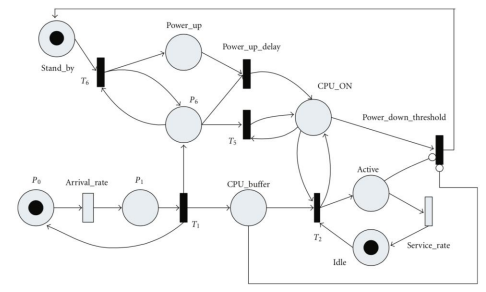
\includegraphics[width=0.9\textwidth, center]{rdp_enun.png}
        \caption{Red de Petri mono-núcleo}
    \end{figure} \newpage
    %%%%%%%%%%%%%%%%%%%%%%%%%%%%%%%%%%%%%%%%%%%%%%%%%%%%%%%%%%%%%%%%%%%%%%%%%%%%%%%%%%%%%%%%
    \section{Implementación y resultados}
    %%%%%%%%%%%%%%%%%%%%%%%%%%%%%%%%%%%%%%%%%%%%%%%%%%%%%%%%%%%%%%%%%%%%%%%%%%%%%%%%%%%%%%%%
    \subsection{Red de Petri}
    En la \emph{figura 2} se observa cómo fue modelada la red de Petri de acuerdo al enunciado. \par
    La red de Petri modelada cuenta con:
    \begin{itemize}
        \item 16 plazas
        \item 15 transiciones
    \end{itemize}
    \begin{figure}[h]
        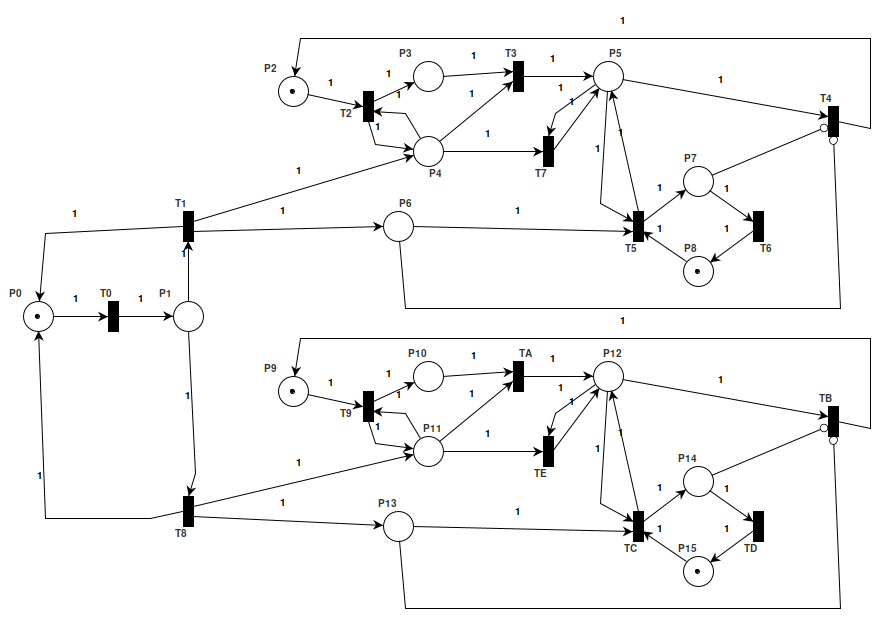
\includegraphics[width=0.9\textwidth, center]{rdp.png}
        \caption{Red de Petri doble núcleo}
    \end{figure}   
    %%%%%%%%%%%%%%%%%%%%%%%%%%%%%%%%%%%%%%%%%%%%%%%%%%%%%%%%%%%%%%%%%%%%%%%%%%%%%%%%%%%%%%%%
    \subsection{Hilos}
    Teniendo en cuenta la red de la \emph{figura 2}, lo siguiente es pensar cuántos hilos
    serán los encargados de ejecutarse el programa. \par
    Luego de realizar un análisis, se llegó a la conclusión de que en la red deben trabajar
    \textbf{7 hilos} en forma concurrente. Estos hilos son llamados:
    \begin{itemize}
        \item ProcessGenerator
        \item CPUPower x 2
        \item CPUProcessing x 2
        \item CPUGarbageCollector x 2
    \end{itemize}
    \textbf{ProcessGenerator:} Encargado de generar los procesos comúnes a ambos CPUs. 
    Dispara las transiciones 0, 1 y 8. \newline \newline
    \textbf{CPUPower:} Maneja el encendido/apagado de cada CPU. Dispara las transiciones
    2, 3 y 4 o 9, A y B. \newline \newline
    \textbf{CPUProcessing:} Procesa las tareas de cada CPU. Dispara las transiciones
    2, 3 y 4 o 9, A y B. \newline \newline
    \textbf{CPUGarbageCollector:} Previene que la plaza número 4/11 no junte \emph{tokens}
    "basura". \newline
    %%%%%%%%%%%%%%%%%%%%%%%%%%%%%%%%%%%%%%%%%%%%%%%%%%%%%%%%%%%%%%%%%%%%%%%%%%%%%%%%%%%%%%%%
    \subsection{Clases en Java}
    El programa encargado de simular el sistema se desarrola en el lenguaje de programación
    \emph{Java}. \par
    A continuación, se describen las clases, implementadas en dicho lenguaje,
    que modelan el programa:
    \begin{itemize}
        \item \textbf{Cola:} Colas (\emph{queues}), las cuales son usadas para que los
        hilos puedan dormir en caso que lo necesiten
        \item \textbf{Colors:} Clase sin funciones que contiene códigos de colores (para 
        loggear)
        \item \textbf{CPUGarbageCollector:} Modelo del hilo CPUGarbageCollector anteriormente
        descrito
        \item \textbf{CPU:} Modela un CPU. Clase encargada de "comunicar" los hilos Generator,
        Processing y GarbageCollector
        \item \textbf{CPUPower:} Modelo del hilo CPUPower anteriormente descrito
        \item \textbf{CPUProcessing:} Modelo del hilo CPUProcessing anteriormente descrito
        \item \textbf{InvarianteTest:} Implementación de un test de t-invariantes
        \item \textbf{Main:} Clase principal y ejecutable
        \item \textbf{Monitor:} Encargada de administrar los tiempos y el uso de la red de 
        Petri
        \item \textbf{Politica:} A la hora de despertar un hilo, la politica es quien decide
        a cuál hacerlo
        \item \textbf{ProcessBuffer:} Modelo de un buffer en el cuál se depositan Process
        \item \textbf{ProcessGenerator:} Modelo del hilo ProcessGenerator anteriormente
        descrito
        \item \textbf{Process:} Clase que simula un proceso de CPU. Dichos Process van a
        parar a un ProcessBuffer
        \item \textbf{RedDePetri:} Implementación de la red de Petri
        \item \textbf{XMLParser:} Parsea las características de la red de Petri desde un
        archivo \emph{xml}
    \end{itemize} \par
    Para información más detallada acerca de las clases y sus funciones, se puede consultar
    la documentación\footnote{\fndoc} hecha por \emph{Doxygen}\footnote{\fndoxy}.
    %%%%%%%%%%%%%%%%%%%%%%%%%%%%%%%%%%%%%%%%%%%%%%%%%%%%%%%%%%%%%%%%%%%%%%%%%%%%%%%%%%%%%%%%
    \subsection{Politica}
    La clase \emph{politica} se encarga de facilitar la elección de a qué hilo despertar en 
    el caso en que haya más de uno durmiendo. \par
    La forma de hacer esto es mediante prioridades: se le asigna una prioridad \textbf{distinta}
    a cada una de las transiciones de la red. \par
    Cuando querramos hacer uso de la politica, simplemente le indicamos cuáles son las
    transiciones listas para dispararse y ella nos indicará cuál de esas transiciones es la
    que tiene la mayor prioridad. \par
    Además, la clase \emph{politica} cuenta con un método capaz de intercambiar prioridades
    entre dos transiciones. Esto podría ser útil, en el caso en que se quiera depositar más
    tareas en un CPU que en el otro.
    %%%%%%%%%%%%%%%%%%%%%%%%%%%%%%%%%%%%%%%%%%%%%%%%%%%%%%%%%%%%%%%%%%%%%%%%%%%%%%%%%%%%%%%%
    \subsection{Invariantes}
    Sabemos que una de las maneras de chequear que la red (y nuestro programa) funciona 
    de forma correcta, es analizando las invariantes. Estas son, las \textbf{t-invariantes}
    y las \textbf{p-invariantes}. \par
    Para el análisis, se usó la herramienta Pipe\footnote{\fnpipe}.
    Los resultados fueron los siguientes: \newline \newline
    \textbf{P-Invariantes:} \\
    \begin{figure}[h]
        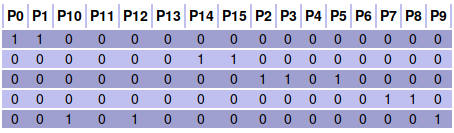
\includegraphics[width=0.7\textwidth, center]{p-invariante.png}
        \caption{Análisis de P-Invariantes en Pipe}
    \end{figure}
    La \emph{figura 3} nos enseña qué plazas están relacionadas mediante una invariante de
    plazas. Esta relación indica que la suma de los \emph{tokens} en dichas plazas, en cada
    relación, sea siempre unitaria. Estos es: \newline \newline
    \begin{center}
        $M(P0) + M(P1) = 1$ \newline \newline
        $M(P14) + M(P15) = 1$ \newline \newline
        $M(P2) + M(P3) + M(P5) = 1$ \newline \newline
        $M(P10) + M(P12) + M(P9) = 1$ \newline \newline
    \end{center} \par
    Para comprobar que lo anterior se cumpla siempre, la clase \emph{RedDePetri} hace un 
    chequeo cada vez que se dispara una transición. El método de la clase que hace dicho
    chequeo se llama \emph{isPInvariantesCorrecto}. \newline \newline
    \textbf{T-Invariantes:} \newline \newline
    De la misma forma, podemos observar en la \emph{figura 4} las invariantes de transición
    que existen en nuestro sistema. \\
    \begin{figure}[h]
        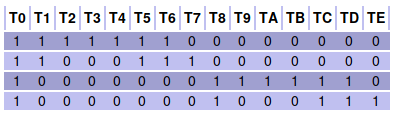
\includegraphics[width=0.7\textwidth, center]{t-invariante.png}
        \caption{Análisis de T-Invariantes en Pipe}
    \end{figure}   
    Anteriormente se mencionó la clase \emph{InvarianteTest}. Esta clase es la encargada
    de chequear, una vez finalizada la ejecución, que el orden de los disparos (de las 
    transiciones) sea el correcto. \par
    Para esto, la clase \emph{Main} se encarga de grabar todas las transiciones (en orden) 
    que han sido disparadas en un archivo\footnote{\fninv} de texto. Luego, la
    clase \emph{InvarianteTest} usa esa información para, mediante un algoritmo de remplazo,
    ir eliminando las coincidencias (o \emph{matches}) entre el \emph{log} de transiciones y
    las invariantes. Si el sistema funciona correctamente, deben quedar eliminadas todas las
    transiciones. De lo contrario, existen errores, que son escritos en otro 
    archivo\footnote{\fninverr} de texto. \newline \newline
    \textbf{Resultados:} \newline \newline \par
    Al finalizar una ejecución, se loggea el estado de los análisis de invariantes. Un ejemplo
    se puede ver en la \emph{figura 5}. \par
    \begin{figure}[h]
        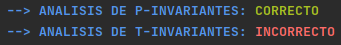
\includegraphics[width=0.5\textwidth, center]{analisis-invariantes-ej.png}
        \caption{Ejemplo del análisis de invariantes de una ejecución}
    \end{figure}
    Se hicieron pruebas\footnote{\fnpruebas} con 100, 1000 y 2000 procesos y con ambos procesos trabajando en forma
    equilibrada (mismo tiempo de procesamiento). Además, se realizaron 10 muestras por cada 
    cantidad de procesos. Los resultados, en la \emph{tabla 1}.\newline \newline
    \begin{center}
        \begin{table}[h]
            \begin{tabular}{||c|c|c||} 
                \hline
                Procesos & Transiciones totales (\emph{avg}) & Transiciones restantes (\emph{avg}) \\ [0.5ex] 
                \hline\hline
                100 & 552,6 & 11,5 \\ 
                \hline
                1000 & 5538,4 & 13,8 \\
                \hline
                2000 & 11061 & 14 \\
                \hline
            \end{tabular}
            \caption{Resultados de análisis. Cada fila equivale a 10 muestras}
        \end{table}
    \end{center} \par
    Como se dijo antes, para que los chequeos sean positivos, la cantidad de transiciones restantes
    debe ser nula. \par
    Claramente, los chequeos de t-invariantes son negativos, siendo esto, obviamente, no deseado. \\
    Sin embargo, la cantidad de transiciones restantes (que no cumplen con una invariante) es 
    relativamente la misma para todos los casos. Esto quiere decir que la cantidad de transiciones
    restantes no dependen de la cantidad de transiciones totales.
    %%%%%%%%%%%%%%%%%%%%%%%%%%%%%%%%%%%%%%%%%%%%%%%%%%%%%%%%%%%%%%%%%%%%%%%%%%%%%%%%%%%%%%%%
    \subsection{Tiempos}
    A continuación, en la \emph{tabla 2}, se describen los tiempos que lleva el programa en 
    ejecutarse. Los tiempos de la red son los siguientes: \par
    \begin{itemize}
        \item \emph{ArrivalRate} = 10 [ms]
        \item \emph{ServiceRate} = 15 [ms]
        \item \emph{StandByDelay} = 30 [ms]
    \end{itemize}
    Se observa una clara linealidad a medida que aumenta la cantidad de procesos. \par
    \begin{center}
        \begin{table}[h]
            \centering
            \begin{tabular}{||c|c||} 
                \hline
                Procesos & Tiempo de ejecución (\emph{avg}) \\ [0.5ex] 
                \hline\hline
                500 & 2,59 \\ 
                \hline
                1000 & 5,16 \\
                \hline
                1500 & 7,76 \\
                \hline
                2000 & 10,35 \\
                \hline
                2500 & 12,95 \\
                \hline
                3000 & 15,53 \\
                \hline
                3500 & 18,13 \\
                \hline
                4000 & 20,74 \\
                \hline
            \end{tabular}
            \caption{Resultados de análisis. Cada fila equivale a 5 muestras}
        \end{table}
    \end{center}
    \begin{figure}[h]
        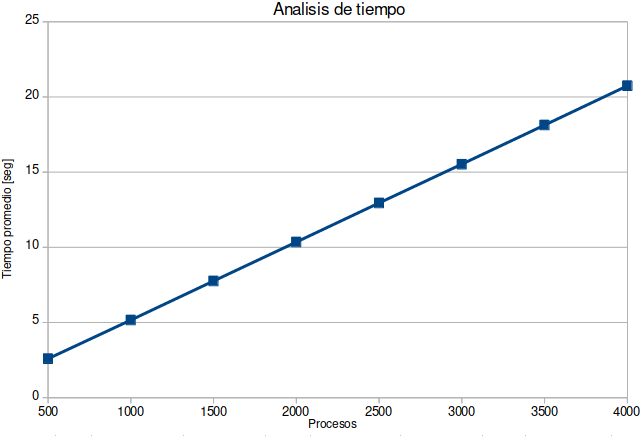
\includegraphics[width=0.9\textwidth, center]{tiempos.png}
        \caption{Gráfica de cantidad de procesos vs tiempos}
    \end{figure}
\end{document}